\section{Codabench}
{{\footnotesize
\begin{description}[labelwidth=5em, labelsep=1em, leftmargin=*, align=left, itemsep=0.3em, parsep=0em]
  \item[date:] 2022-01-01
  \item[last\_updated:] 2025-03
  \item[expired:] unkown
  \item[valid:] yes
  \item[url:] \href{https://www.codabench.org/}{https://www.codabench.org/}
  \item[domain:] General ML; Multiple
  \item[focus:] Open-source platform for organizing reproducible AI benchmarks and competitions
  \item[keywords:]
    - benchmark platform
    - code submission
    - competitions
    - meta-benchmark
  \item[task\_types:]
    - Multiple
  \item[ai\_capability\_measured:]
    - Model reproducibility
    - performance across datasets
  \item[metrics:]
    - Submission count
    - Leaderboard ranking
    - Task-specific metrics
  \item[models:]
    - Arbitrary code submissions
  \item[ml\_motif:]
    - Multiple
  \item[type:] Platform
  \item[ml\_task:] Multiple
  \item[notes:] Hosts 51 public competitions, \textasciitilde{}26 k users, 177 k submissions :contentReference[oaicite:2]\{index=2\}
  \item[contact.name:] Isabelle Guyon (Université Paris-Saclay)
  \item[contact.email:] unkown
  \item[results.name:] ChatGPT LLM
  \item[results.url:] \href{unkown}{unkown}
  \item[fair.reproducible:] Yes
  \item[fair.benchmark\_ready:] Yes
  \item[ratings.software.rating:] 0
  \item[ratings.software.reason:] Not analyzed.
  \item[ratings.specification.rating:] 10.0
  \item[ratings.specification.reason:] Simulation task (generative calorimeter showers) is clearly stated with multiple datasets, fidelity requirements, and performance constraints.
  \item[ratings.dataset.rating:] 9.5
  \item[ratings.dataset.reason:] Public datasets available in multiple sizes and formats; well-documented; not versioned
  \item[ratings.metrics.rating:] 10.0
  \item[ratings.metrics.reason:] Histogram similarity, classifier AUC, and generation latency are clearly defined and benchmarked across all submissions.
  \item[ratings.reference\_solution.rating:] 9.0
  \item[ratings.reference\_solution.reason:] 31 model implementations submitted; some made public and reproducible, though others remain undocumented or private.
  \item[ratings.documentation.rating:] 9.0
  \item[ratings.documentation.reason:] Paper, leaderboard, and Gemini doc are comprehensive; unified repo or launchable baseline kit would push this to a 10.
  \item[id:] codabench
  \item[Citations:] \cite{xu-2022}
  \item[Ratings:]
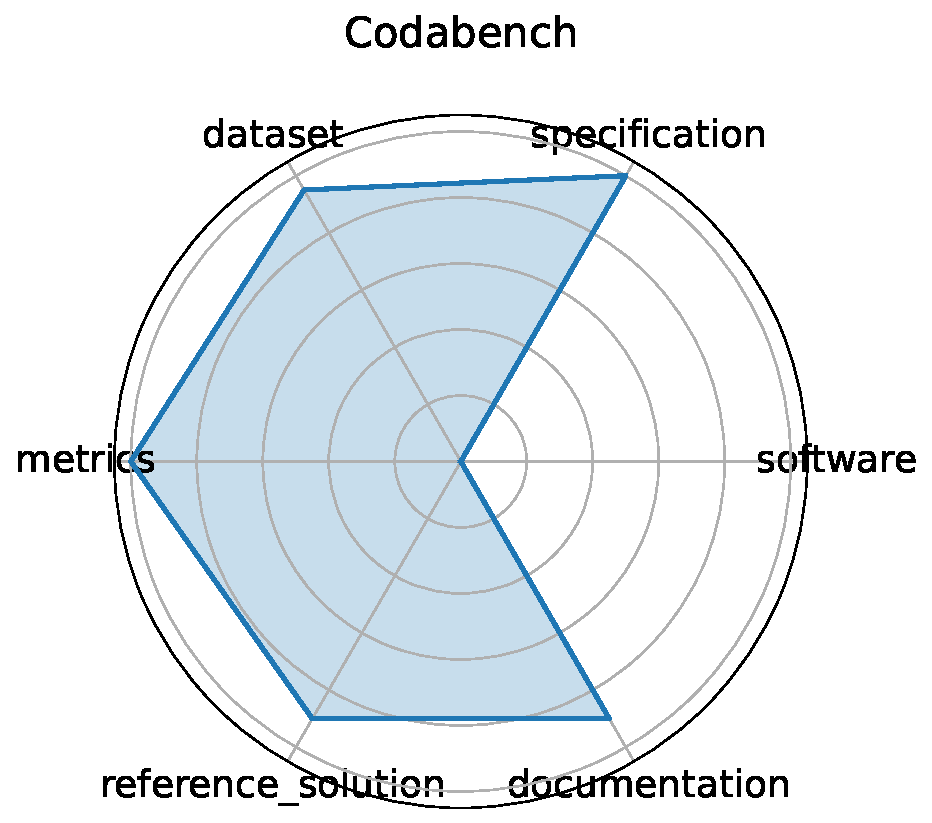
\includegraphics[width=0.2\textwidth]{codabench_radar.pdf}
\end{description}
}}
\clearpage